\newpage
\section{Exercices}
 {\small
  \begin{multicols}{2}
	  \begin{exo}
	On choisit au hasard un jour de l'année.

	On considère les événements :
	\begin{itemize}
		\item $P$ : \og{} le jour choisi a été pluvieux \fg{}
		\item $V$ : \og{} le jour choisi a été venté \fg{}
	\end{itemize}
	Pour chacune des informations suivantes, indiquer si elle correspond, ou non, à une probabilité conditionnelle, et donner la notation correspondant à cette probabilité.
	\begin{enumerate}
		\item Dans l'année, $40$\% des jours sont pluvieux.
		\item $66$\% des jours pluvieux sont ventés.
		\item Parmi les jours non ventés, $22$\% sont pluvieux.
		\item $49$\% des jours dans l'année n'ont été ni ventés, ni pluvieux.
	\end{enumerate}
\end{exo}

	  \begin{exo}
	On choisit une personne au hasard dans un groupe constitué de garçons et de filles.

	On considère les événements suivants :
	\begin{itemize}
		\item $F$ : \og{} la personne est une fille \fg{}
		\item $S$ : \og{} la personne pratique un sport en club \fg{}
	\end{itemize}
	\begin{enumerate}
		\item Traduire les propositions suivantes en utilisant les notations de probabilités :
		      \begin{enumerate}
			      \item Dans ce groupe il y a $8$\% de filles qui font du sport en club.
			      \item Le sport est pratiqué en club pour $40$\% des garçons.
			      \item Il y a $32$\% des personnes qui font du sport en club.
			      \item Parmi ceux qui pratiquent un sport en club, il y a $25$\% de filles.
		      \end{enumerate}
		\item Traduire en langage naturel les égalités :\vspace*{-2mm}
		      \[
			      P\pa{\bar{F} \cap S} = 0,24\quad\text{et}\quad P_{S}\pa{\bar{F}} = 0,75
		      \]

	\end{enumerate}
\end{exo}

	  \begin{exo}
	Dans un stock de pommes provenant de deux fournisseurs ($A$ et $B$), on prend au hasard une pomme. 

	On note :
	\begin{itemize}
		\item $A$ : \og{} La pomme provient du fournisseur $A$ \fg{}
		\item $C$ : \og{} La pomme est commercialisable \fg{}.
	\end{itemize}
	
	On sait que $83$\% des pommes provenant du fournisseur $A$ sont commercialisables.

	En utilisant les événements $A$ et $C$, compléter avec une probabilité :\vspace*{-2mm} $$\ldots \ldots \ldots = 0,83$$
\end{exo}

	  \begin{exo}
	On considère deux événements $R$ et $S$ tels que :
	\[
		P(R) = \dfrac{1}{4}\ ,\quad P_{R}(S) = \dfrac{5}{6}\quad\text{et}\quad P_{\overline{R}}\left(\overline{S}\right) = \dfrac{11}{12}
	\]

	Construire un arbre pondéré avec $R$ et $S$.
\end{exo}

	  \vfill~\columnbreak
	  \begin{exo}
	Dans l'arbre ci-dessous, exprimer chacune des pondérations comme une probabilité (par ex. $0,65 = P_{A}\left(\overline{B}\right)$)

	\begin{center}
		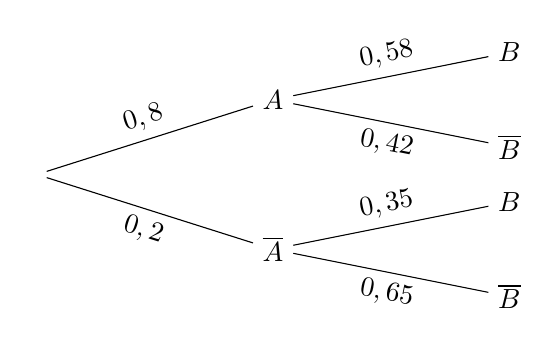
\begin{tikzpicture}[grow=right,sloped, level distance=3cm,
				level 1/.style={sibling distance=1.9cm},
				level 2/.style={sibling distance=1.2cm}]
			\node {}
			child {node {$\overline{A}$}
					child {node {$\overline{B}$} edge from parent node[below] {$0,65$}}
					child {node {$B$} edge from parent node[above] {$0,35$}}
					edge from parent node[below] {$0,2$}
				}
			child {node {$A$}
					child {node {$\overline{B}$} edge from parent node[below] {$0,42$}}
					child {node {$B$} edge from parent node[above] {$0,58$}}
					edge from parent node[above] {$0,8$}
				};
		\end{tikzpicture}
	\end{center}
\end{exo}

	  \begin{exo}
	Dans un lycée, $60$\% des élèves ont une calculatrice graphique dont $80$\% sont de marque $A$.

	Si la calculatrice n'est pas graphique, alors elle est de marque $A$ dans $50$\% des cas.

	On emprunte la calculatrice d'un élève au hasard et on considère les événements suivants :
	\begin{itemize}
		\item $G$ : \og{} Sa calculatrice est graphique. \fg{}
		\item $A$ : \og{} Sa calculatrice est de marque $A$ \fg{}
	\end{itemize}

	\begin{enumerate}
		\item Modéliser la situation à l'aide d'un arbre pondéré mettant en jeu les événements $G$ et $A$.
		      % \item Quelle est la probabilité que ce soit une calculatrice graphique de marque $A$ ?
	\end{enumerate}
	\begin{center}
		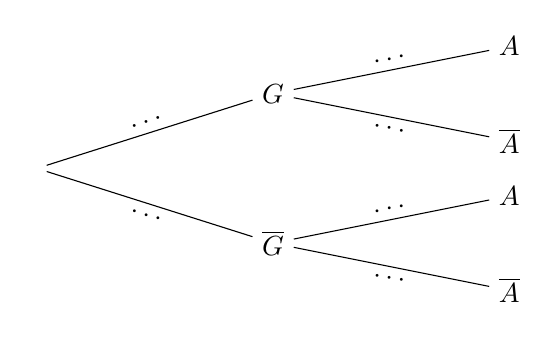
\begin{tikzpicture}[grow=right,sloped, level distance=3cm,
				level 1/.style={sibling distance=1.9cm},
				level 2/.style={sibling distance=1.2cm}]
			\node {}
			child {node {$\overline{G}$}
					child {node {$\overline{A}$} edge from parent node[below] {$\ldots$}}
					child {node {$A$} edge from parent node[above] {$\ldots$}}
					edge from parent node[below] {$\ldots$}
				}
			child {node {$G$}
					child {node {$\overline{A}$} edge from parent node[below] {$\ldots$}}
					child {node {$A$} edge from parent node[above] {$\ldots$}}
					edge from parent node[above] {$\ldots$}
				};
		\end{tikzpicture}
	\end{center}

\end{exo}

	  \begin{exo}
	On étudie une population de $100$ individus selon deux caractères $A$ (et son contraire $\overline{A}$) ainsi que $B$ (et son contraire $\overline{B}$).

	\begin{enumerate}
		\item Compléter le tableau des effectifs ci-dessous à l'aide des informations fournies :
		      \begin{itemize}
			      \item L'effectif associé à l'événement $A$ est de $60$.
			      \item L'effectif de l'intersection $A \cap B$ est de $25$.
			      \item L'effectif associé à l'événement $\overline{B}$ est de $45$.
		      \end{itemize}
	\end{enumerate}
	\begin{center}
		\renewcommand{\arraystretch}{1.2}
		\begin{tabular}{|c|C{2cm}|C{2cm}|c|}
			\hline
			               & $B$  & $\overline{B}$ & \textbf{Total} \\ \hline
			$A$            & $25$ &                & $60$           \\ \hline
			$\overline{A}$ &      &                &                \\ \hline
			\textbf{Total} &      & $45$           & $100$          \\ \hline
		\end{tabular}
	\end{center}
\end{exo}

	  \vfill~\columnbreak
	  \begin{exo}
	Dans une classe de $32$ élèves, il y a $15$ garçons et $28$ demi-pensionnaires. $12$ garçons sont demi-pensionnaires.

	% On choisit un élève de cette classe au hasard.
	% \begin{enumerate}

	Compléter le tableau des effectifs à double entrée en fonction de ces deux critères.
	% \end{enumerate}

	\begin{center}
		\renewcommand{\arraystretch}{1.2}
		\begin{tabular}{|c|C{1cm}|C{1cm}|c|} \hline
			                 & \textbf{DP}  & \textbf{Ext.} & \textbf{Total} \\ \hline
			\textbf{Garçons} & \phantom{12} & \phantom{3}   & \phantom{15}   \\ \hline
			\textbf{Filles}  & \phantom{16} & \phantom{1}   & \phantom{17}   \\ \hline
			\textbf{Total}   & \phantom{28} & \phantom{4}   & \phantom{32}   \\ \hline
		\end{tabular}
	\end{center}
\end{exo}

	  \begin{exo}
	On considère une urne contenant deux boules rouges et cinq boules vertes. On effectue deux tirages successifs au hasard \textbf{sans remise}.

	On note $R_i$ l'événement "On a tiré une boule rouge au i-ième tirage" et $V_i$ l'événement "on a tiré une boule verte au i-ième tirage".
	
	Construire un arbre pondéré représentant cette situation, puis calculer la probabilité de tirer deux boules rouges.
\end{exo}

	  \begin{exo}
	Une entreprise de jouets est spécialisée dans la fabrication de poupées qui parlent et qui marchent.

	Chaque poupée peut présenter deux défauts et deux seulement : un défaut mécanique, un défaut électrique.

	Une étude statistique montre que :
	\begin{itemize}
		\item $8$\% des poupées présentent le défaut mécanique ;
		\item $5$\% des poupées présentent le défaut électrique ;
		\item $2$\% des poupées présentent ces deux défauts.
	\end{itemize}

	La production journalière est de $\np{1000}$ poupées.

	À l'aide des données du texte, organiser l'ensemble de la production journalière en construisant et en complétant un tableau d'effectifs à double entrée.
\end{exo}

	  \begin{exo}
	Dans le tableau ci-dessous, on note :
	\begin{itemize}
		\item $F$ : \og{} La personne est une fille \fg{}
		\item $V$ : \og{} La personne a plus de 20 ans \fg{}
	\end{itemize}

	On choisit une personne au hasard dans ce groupe.

	\begin{center}
		\renewcommand{\arraystretch}{1.2}
		\begin{tabular}{|c|C{2cm}|C{2cm}|c|}
			\hline
			               & $F$ & $\overline{F}$ & \textbf{Total} \\ \hline
			$V$            & 6   & 44             & 50             \\ \hline
			$\overline{V}$ & 56  & 59             & 115            \\ \hline
			\textbf{Total} & 62  & 103            & 165            \\ \hline
		\end{tabular}
	\end{center}

	À l'aide du tableau, déterminer les probabilités suivantes (on donnera les résultats sous forme de fraction) :

	\begin{enumerate}
		\item \textbf{Proba. marginales :} $P\pa{F}$ et $P\pa{V}$
		\item \textbf{Proba. d'intersection :} $P\pa{F \cap V}$ et $P\pa{\overline{F} \cap \overline{V}}$
		\item \textbf{Proba. conditionnelles :} $P_{V}\pa{\overline{F}}$ et $P_{F}\pa{V}$
	\end{enumerate}
\end{exo}

	  \vfill~\columnbreak
	  \begin{exo}
	Dans une boulangerie, on dispose d'une réduction si l'on choisit la formule \og{} dessert mystère \fg{} pour laquelle le dessert accompagnant le menu est tiré au hasard.

	Ceyda choisit cette formule alors que les desserts encore disponibles sont répartis comme suit :

	\begin{center}
		\renewcommand{\arraystretch}{1.2}
		\begin{tabular}{|c|c|c|c|} \hline
			           & Chocolat     & Vanille     & Total        \\ \hline
			Tartelette & \phantom{8}  & 11          & 19           \\ \hline
			Éclair     & \phantom{13} & \phantom{7} & \phantom{20} \\ \hline
			Total      & \phantom{21} & 18          & 39           \\ \hline
		\end{tabular}
	\end{center}

	On considère les événements $E$ : \og{} Son dessert est un éclair \fg{} et $V$ : \og{} Son dessert est à la vanille. \fg{}

	\begin{enumerate}
		\item Calculer $p_{E}(V)$, $p_{V}(E)$, $p_{\overline{E}}(V)$.
		\item Ceyda voit que son dessert est un éclair.

		      Écrire la probabilité qu'il soit au chocolat comme une probabilité conditionnelle puis la calculer.
	\end{enumerate}
\end{exo}

	  \begin{exo}
	On étudie une population d'individus selon deux caractères distincts traduits par les événements $A$ et $B$.

	\begin{enumerate}
		\item Compléter le tableau d'effectifs :

		      \begin{center}
			      \renewcommand{\arraystretch}{1.2}
			      \begin{tabular}{|c|C{2cm}|C{2cm}|c|} \hline
				                     & $B$  & $\overline{B}$ & \textbf{Total} \\ \hline
				      $A$            &      &                & $80$           \\ \hline
				      $\overline{A}$ & $30$ &                &                \\ \hline
				      \textbf{Total} &      & $110$          & $200$          \\ \hline
			      \end{tabular}
		      \end{center}
	\end{enumerate}

	On choisit un individu au hasard dans cette population.

	\ber
	\item Déterminer les probabilités suivantes :
	\begin{enumerate}
		\item $P\pa{\bar{A}}$
		\item $P\pa{A \cap \bar{B}}$ et $P\pa{\overline{A} \cap \overline{B}}$
		\item $P_{B}\pa{A}$ et $P_{A}\pa{\overline{B}}$
	\end{enumerate}
	\end{enumerate}
\end{exo}

	  \begin{exo}
	On considère l'arbre de probabilités ci-dessous représentant une situation aléatoire mettant en jeu deux événements $A$ et $B$.

	\begin{center}
		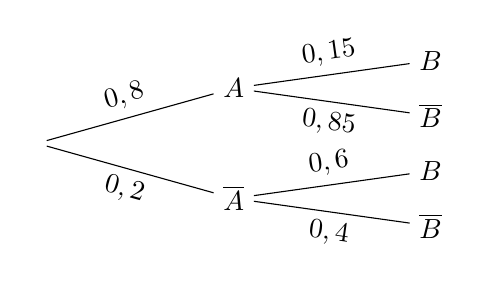
\begin{tikzpicture}[grow=right, sloped, level distance=2.5cm, level 1/.style={sibling distance=1.4cm}, level 2/.style={sibling distance=0.7cm}]
			\node {}
			child {node {$\overline{A}$}
					child {node {$\overline{B}$} edge from parent node[below] {$0,4$}}
					child {node {$B$} edge from parent node[above] {$0,6$}}
					edge from parent node[below] {$0,2$}
				}
			child {node {$A$}
					child {node {$\overline{B}$} edge from parent node[below] {$0,85$}}
					child {node {$B$} edge from parent node[above] {$0,15$}}
					edge from parent node[above] {$0,8$}
				};

		\end{tikzpicture}
	\end{center}

	\begin{enumerate}
		\item Par lecture directe sur l'arbre, donner les valeurs des probabilités suivantes :
		      \[
			      P(A)\ ,\ P_{A}(\overline{B})\ \text{ et }\ P_{\overline{A}}(B)
		      \]

		\item Calculer la probabilité des événements :
		      \[
				  A \cap B\ \text{ et }\ \bar{A} \cap B
		      \]

	\end{enumerate}
\end{exo}

	  \vfill~\columnbreak
	  \begin{exo}
	Dans un pays européen, $12$\% des moutons sont atteints par une maladie.

	Un test de dépistage de cette maladie vient d'être mis sur le marché, mais il n'est pas totalement fiable.

	Une étude a montré que quand le mouton est malade, le test est positif dans 93 \% des cas ; quand le mouton est sain, le test est négatif dans $97$\% des cas.

	On choisit un mouton au hasard et on le soumet au test de dépistage de la maladie.

	On note :
	\begin{itemize}
		\item $M$ l'événement \og{} le mouton est malade \fg{}
		\item $Po$ l'événement \og{} le test est positif \fg{}
	\end{itemize}
	\begin{enumerate}
		\item À l'aide des informations de l'énoncé, donner les valeurs des probabilités suivantes :
		      \[
			      P(M)\ ,\ P_{M}(Po)\ \text{et}\ P_{\overline{M}}(\overline{Po})
		      \]

		\item Compléter l'arbre de probabilité suivant :
	\end{enumerate}
	\begin{center}
		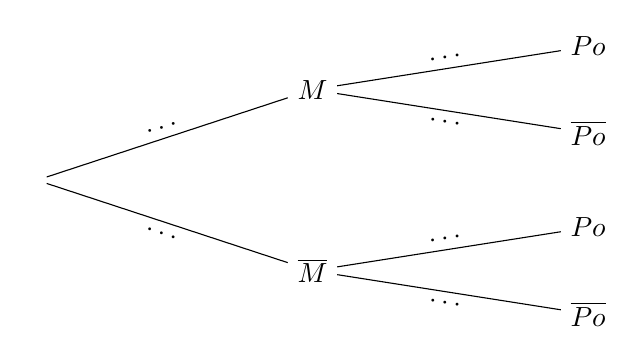
\begin{tikzpicture}[grow=right, sloped, level distance=3.5cm,
				level 1/.style={sibling distance=2.3cm},
				level 2/.style={sibling distance=1.1cm}]

			\node {}
			child {node {$\overline{M}$}
					child {node {$\overline{Po}$} edge from parent node[below] {\dots}}
					child {node {$Po$} edge from parent node[above] {\dots}}
					edge from parent node[below] {\dots}
				}
			child {node {$M$}
					child {node {$\overline{Po}$} edge from parent node[below] {\dots}}
					child {node {$Po$} edge from parent node[above] {\dots}}
					edge from parent node[above] {\dots}
				};

		\end{tikzpicture}
	\end{center}

	\begin{enumerate}[resume]
		\item Calculer $P\pa{M\cap Po}$ et interpréter le résultat dans le cadre de l'exercice.
		\item Calculer la probabilité que le mouton soit sain et que son test soit négatif.
	\end{enumerate}
\end{exo}

	  \begin{exo}
	$A$ et $B$ sont deux événements d'une même situation aléatoire, et on donne :
	\[
		P(A) = \frac{7}{12} \quad ; \quad P(B) = \frac{5}{12} \quad \text{et} \quad P(A \cup B) = \frac{3}{4}
	\]

	\begin{enumerate}
		\item À l'aide de la formule du cours reliant l'union et l'intersection, calculer $P\pa{A \cap B}$.
		\item En déduire les probabilités conditionnelles $P_{A}\pa{B}$ et $P_{B}\pa{A}$. Les résultats seront donnés sous forme de fractions irréductibles.
	\end{enumerate}

	\noindent\textbf{Rappel :} Pour deux événements quelconques $A$ et $B$ d'une même situation aléatoire, la probabilité de leur union est donnée par :
	\[
		P(A \cup B) = P(A) + P(B) - P(A \cap B)
	\]

\end{exo}

	  \vfill~\columnbreak
	  \begin{exo}
	On considère deux événements $A$ et $B$ d'une même situation aléatoire tels que :
	\[
		P(A) = 0,3 \quad ; \quad P(B) = 0,6 \quad \text{et} \quad P(A \cap B) = 0,2
	\]

	\begin{enumerate}
		\item Rappeler la formule du cours qui permet de calculer la probabilité conditionnelle $P_{A}\pa{B}$ à l'aide de $P\pa{A}$ et de $P\pa{A \cap B}$.
		\item Calculer la probabilité que l'événement $B$ se réalise sachant que l'événement $A$ est réalisé.
		\item Calculer de la même manière la probabilité conditionnelle $P_{B}\pa{A}$.
	\end{enumerate}
\end{exo}

	  \begin{exo}
	Dans une étude statistique, on considère une classe de 24 élèves où chaque élève est représenté par une case dans le graphique ci-dessous :

	\begin{center}
		\begin{tikzpicture}[scale=0.7]
			\fill[black!30] (0,0) rectangle (2,4);
			\fill[pattern=north east lines] (0,1) rectangle (1,4);
			\fill[pattern=north east lines] (1,2) rectangle (2,4);
			\fill[pattern=north east lines] (2,3) rectangle (6,4);
			\draw[step=1cm, black, thin] (0,0) grid (6,4);
		\end{tikzpicture}
		\hfill
		\begin{tikzpicture}[scale=0.6, every node/.style={scale=0.9}]
			\draw[fill=black!30] (0,1.2) rectangle (1.5,1.7) node[right, black, midway, xshift=0.9cm] {Garçon};
			\draw[pattern=north east lines] (0,0.3) rectangle (1.5,0.8) node[right, black, midway, xshift=0.9cm] {Demi-pensionnaire};
		\end{tikzpicture}
	\end{center}

	Deux caractères sont étudiés chez les individus de cette étude :
	\begin{itemize}
		\item $G$ : \og{} l'élève est un garçon \fg{} ;
		\item $D$ : \og{} l'élève est demi-pensionnaire \fg{}.
	\end{itemize}

	L'expérience aléatoire consiste à choisir un élève au hasard dans la classe et de regarder la réalisation ou non de ces deux critères.
	\begin{enumerate}
		\item Compléter l'arbre de probabilité ci-dessous.
	\end{enumerate}

	\begin{center}
		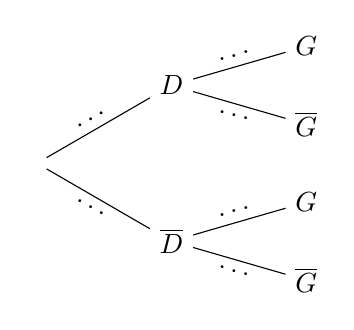
\begin{tikzpicture}[grow=right, sloped, level distance=1.9cm,
				level 1/.style={sibling distance=2.2cm},
				level 2/.style={sibling distance=1.1cm},
				scale=0.9]

			\node {}
			child {node {$\overline{D}$}
					child {node {$\overline{G}$} edge from parent node[below] {\dots}}
					child {node {$G$} edge from parent node[above] {\dots}}
					edge from parent node[below] {\dots}
				}
			child {node {$D$}
					child {node {$\overline{G}$} edge from parent node[below] {\dots}}
					child {node {$G$} edge from parent node[above] {\dots}}
					edge from parent node[above] {\dots}
				};
		\end{tikzpicture}
	\end{center}

	\begin{enumerate}[resume]
		\item Donner par lecture directe la valeur des probabilités suivantes :
		      \[
			      P(D),\ P_{D}(G)\ \text{et}\ P_{\overline{D}}(\overline{G})
		      \]

		\item Calculer la probabilité de l'événement $G \cap \overline{D}$.
		\item Calculer la probabilité que l'élève choisi soit une fille demi-pensionnaire.
		\item Sachant que l'élève choisi est un garçon, quelle est la probabilité qu'il soit demi-pensionnaire ?
	\end{enumerate}
\end{exo}

	  \vfill~\columnbreak
	  \begin{exo}
	Dans un magasin de meubles, le stock est composé de deux types de meubles :
	\begin{itemize}
		\item $60$\% de canapés et le reste est constitué de fauteuils.
		\item Parmi les fauteuils, $20$\% sont en cuir.
		\item La proportion totale de meubles en cuir (canapés ou fauteuils) dans le magasin est de $44$\%.
	\end{itemize}
	Un client se présente et choisit un meuble au hasard. On considère les événements suivants :
	\begin{itemize}
		\item $F$ : \og{} le meuble choisi est un fauteuil \fg{} ;
		\item $C$ : \og{} le meuble choisi est en cuir \fg{}.
	\end{itemize}

	\begin{enumerate}
		\item Donner, à l'aide des données de l'énoncé, les valeurs de $P(F)$, $P(C)$ et $P_{F}(C)$.
		\item Déterminer la probabilité $P(F \cap C)$ que le meuble choisi soit un fauteuil et qu'il soit en cuir.
		\item Rappeler la formule reliant $P_{C}(F)$, $P(F \cap C)$ et $P(C)$.
		\item À l'aide de cette formule, calculer la probabilité que le meuble choisi soit un fauteuil sachant qu'il est en cuir.
	\end{enumerate}
\end{exo}

	  \begin{exo}
	Lorsque le basketteur Stephen Curry tire en match, il y a $53$\% de chance que ce soit un tir à $2$ points et $47$\% que ce soit un tir à $3$ points.

	De plus, quand il tire à $2$ points, son pourcentage de réussite est de $51,5$\% contre $43,5$\% à $3$ points.

	Lorsque Curry tire en match, on considère les événements :

	\begin{itemize}
		\item $D$ : \og{} Il tire à $2$ points \fg{}
		\item $M$ : \og{} Il marque. \fg{}
	\end{itemize}

	\begin{enumerate}
		\item Compléter l'arbre pondéré ci-dessous :
	\end{enumerate}

	\begin{center}
		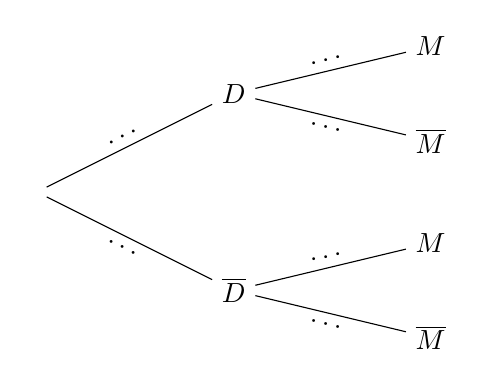
\begin{tikzpicture}[grow=right, sloped, level distance=2.5cm,
				level 1/.style={sibling distance=2.5cm},
				level 2/.style={sibling distance=1.2cm}]

			\node {}
			child {node {$\overline{D}$}
					child {node {$\overline{M}$} edge from parent node[below] {\dots}}
					child {node {$M$} edge from parent node[above] {\dots}}
					edge from parent node[below] {\dots}
				}
			child {node {$D$}
					child {node {$\overline{M}$} edge from parent node[below] {\dots}}
					child {node {$M$} edge from parent node[above] {\dots}}
					edge from parent node[above] {\dots}
				};
		\end{tikzpicture}
	\end{center}
	
	\begin{enumerate}[resume]
		\item Calculer la probabilité que Stephen Curry tente un tir à $2$ points et le marque.
		\item Calculer la probabilité $P\pa{\overline{D} \cap M}$ et interpréter cette valeur dans le contexte de l'exercice.
	\end{enumerate}

	On admet que :
	\[
		P\pa{M} = P\pa{D \cap M} + P\pa{\overline{D} \cap M}
	\]

	\begin{enumerate}[resume]
		\item Calculer la probabilité $P\pa{M}$ qu'il marque son tir.
	\end{enumerate}
\end{exo}

	  \vfill~\columnbreak
	  \begin{exo}
	Dans une ville, une enquête portant sur les habitudes des ménages en matière d'écologie a donné les résultats suivants :
	\begin{itemize}
		\item $70$\% des ménages pratiquent le tri sélectif ;
		\item Parmi les ménages pratiquant le tri sélectif, $40$\% consomment des produits bio ;
		\item Parmi les ménages ne pratiquant pas le tri sélectif, $10$\% consomment des produits bio.
	\end{itemize}

	On choisit un ménage au hasard et on note les événements :

	\begin{itemize}
		\item $T$ : \og{} le ménage pratique le tri sélectif \fg{} ;
		\item $B$ : \og{} le ménage consomme des produits bio \fg{}.
	\end{itemize}

	\begin{enumerate}
		\item \begin{enumerate}
			      \item Déterminer, sans justification, $P(T)$.
			      \item Déterminer, sans justification, les probabilités conditionnelles :
			            \[
				            P_{T}\pa{B}\ \text{ et }\ P_{\overline{T}}\pa{B}
			            \]

		      \end{enumerate}
		\item Représenter la situation à l'aide d'un arbre pondéré.
	\end{enumerate}

	\begin{center}
		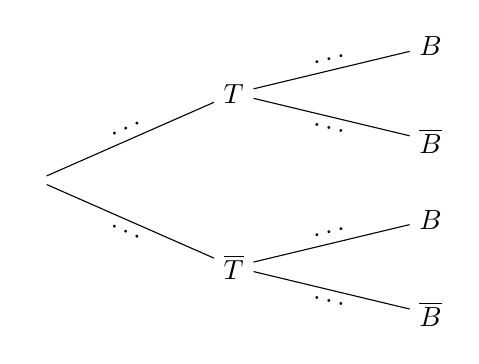
\begin{tikzpicture}[grow=right, sloped, level distance=2.5cm,
				level 1/.style={sibling distance=2.2cm},
				level 2/.style={sibling distance=1.2cm}]

			\node {}
			child {node {$\overline{T}$}
					child {node {$\overline{B}$} edge from parent node[below] {$\ldots$}}
					child {node {$B$} edge from parent node[above] {$\ldots$}}
					edge from parent node[below] {$\ldots$}
				}
			child {node {$T$}
					child {node {$\overline{B}$} edge from parent node[below] {$\ldots$}}
					child {node {$B$} edge from parent node[above] {$\ldots$}}
					edge from parent node[above] {$\ldots$}
				};
		\end{tikzpicture}
	\end{center}

	\ber
	\item
	\begin{enumerate}
		\item Calculer la probabilité de : \og{} le ménage pratique le tri sélectif et consomme des produits bio \fg{}.
		\item Calculer $P\pa{\bar{T}\cap B}$.
	\end{enumerate}
	\end{enumerate}
	L'événement $B$ est formé par la réunion des deux événements incompatibles $T \cap B$ et $\overline{T} \cap B$, on admet que :
	\[ P(B) = P(T \cap B) + P(\overline{T} \cap B) \]
	\ber
	\item Calculer $P\pa{B}$ et vérifier que la probabilité que le ménage consomme des produits bio est égale à $0,31$.
	\item Calculer la probabilité que le ménage pratique le tri sélectif sachant qu'il consomme des produits bio.
	\end{enumerate}
\end{exo}

	  \begin{exo}
	Une entreprise de logistique évalue la performance de ses robots trieurs de colis.

	On étudie un lot de colis à l'aide de deux critères :

	\begin{itemize}
		\item $A$ : \og{} Le colis est fragile \fg{} ;
		\item $B$ : \og{} Le colis est correctement orienté par le robot \fg{}.
	\end{itemize}

	L'ingénieur en chef a mesuré les effectifs mais une partie des données dépend du nombre de robots de type \og{} Alpha \fg{} en activité, noté $n$ (où $n$ est un entier positif).

	\columnbreak

	Le tableau croisé des effectifs est le suivant :

	\begin{center}
		\renewcommand{\arraystretch}{1.2}
		\begin{tabular}{|C{1.5cm}|C{1cm}|C{1cm}|C{1.5cm}|}
			\hline
			               & $B$      & $\overline{B}$ & \textbf{Total} \\ \hline
			$A$            & $n$      & $12$           & $n + 12$       \\ \hline
			$\overline{A}$ & $48$     & $60$           & $108$          \\ \hline
			\textbf{Total} & $n + 48$ & $72$           & $n + 120$      \\ \hline
		\end{tabular}
	\end{center}

	On choisit au hasard un colis dans ce lot.

	\begin{enumerate}
		\item Exprimer en fonction de $n$ les probabilités :
		      \[
			      P(A \cap B)\ \text{et}\ P(B)
		      \]

		\item Rappeler la formule du cours exprimant la probabilité conditionnelle $P_{B}(A)$ en fonction de $P(A \cap B)$ et $P(B)$.
		\item En déduire que la probabilité que le colis soit fragile sachant qu'il est correctement orienté s'exprime par :
		      \[ P_{B}(A) = \frac{n}{n + 48} \]
	\end{enumerate}

	L'ingénieur souhaite que la probabilité qu'un colis correctement orienté soit fragile soit exactement égale à $0,2$ (soit $\frac{1}{5}$).

	\ber
	\item Déterminer la valeur de $n$ pour atteindre cet objectif.
	\end{enumerate}
\end{exo}

	  \vfill~\columnbreak
	  \vfill~
  \end{multicols}
 }
